% Motivating example figure for the introduction.
% Two URIs with parse trees that differ in one production.
% The trace diff is attributable to the differing production.
\documentclass[tikz,border=10pt]{standalone}
\usepackage{tikz}
\usepackage{xcolor}
\usetikzlibrary{positioning,arrows.meta,calc,fit,backgrounds}

\definecolor{hostcol}{HTML}{4A7AB7}
\definecolor{portcol}{HTML}{D97757}
\definecolor{pathcol}{HTML}{6C8B3F}
\definecolor{cfgcol}{HTML}{F5F2EA}

\begin{document}
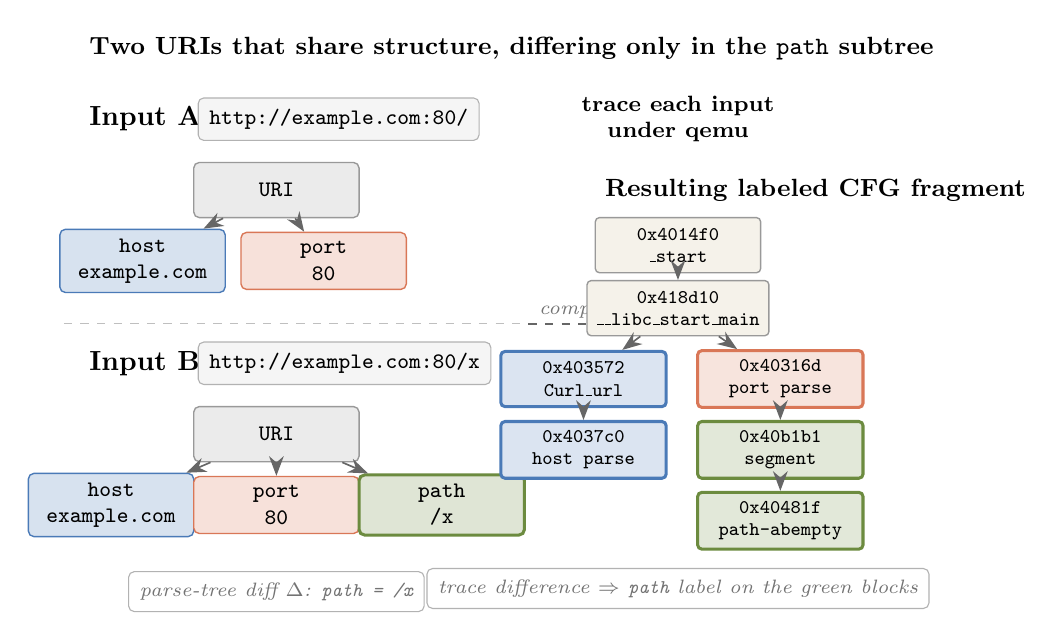
\begin{tikzpicture}[
  font=\sffamily\small,
  prod/.style={
    rounded corners=2pt, minimum height=0.7cm, minimum width=2.1cm, align=center,
    line width=0.5pt, font=\footnotesize\ttfamily,
  },
  bb/.style={
    draw=black!40, fill=cfgcol, line width=0.5pt,
    rounded corners=1.5pt,
    minimum height=0.7cm, minimum width=2.1cm, align=center,
    font=\scriptsize\ttfamily,
  },
  bblabeled/.style={
    bb, draw=#1, fill=#1!20, line width=1.1pt, font=\scriptsize\ttfamily\bfseries,
  },
  arrow/.style={-{Stealth[length=2.5mm]}, line width=0.6pt, draw=black!60},
  cflabel/.style={font=\scriptsize\itshape, text=black!55},
]

% ============================================================
% LEFT COLUMN: two inputs and their parse trees
% ============================================================

% Title
\node[font=\bfseries\small, anchor=west] at (-1.0, 6.5) {Two URIs that share structure, differing only in the \texttt{path} subtree};

% --- Input A ---
\node[font=\bfseries, anchor=west] at (-1.0, 5.6) {Input A};
\node[font=\ttfamily\footnotesize, anchor=west, draw=black!30, fill=black!4,
      rounded corners=2pt, inner sep=4pt] at (0.5, 5.6)
      {http://example.com:80/};

\node[prod, fill=black!8, draw=black!40] (aroot) at (1.5, 4.7) {URI};
\node[prod, draw=hostcol, fill=hostcol!22] (ahost) at (-0.2, 3.8) {host\\example.com};
\node[prod, draw=portcol, fill=portcol!22] (aport) at (2.1, 3.8) {port\\80};
\draw[arrow] (aroot) -- (ahost);
\draw[arrow] (aroot) -- (aport);

% --- Separator ---
\draw[dashed, black!25] (-1.2, 3.0) -- (4.6, 3.0);

% --- Input B ---
\node[font=\bfseries, anchor=west] at (-1.0, 2.5) {Input B};
\node[font=\ttfamily\footnotesize, anchor=west, draw=black!30, fill=black!4,
      rounded corners=2pt, inner sep=4pt] at (0.5, 2.5)
      {http://example.com:80/x};

\node[prod, fill=black!8, draw=black!40] (broot) at (1.5, 1.6) {URI};
\node[prod, draw=hostcol, fill=hostcol!22] (bhost) at (-0.6, 0.7) {host\\example.com};
\node[prod, draw=portcol, fill=portcol!22] (bport) at (1.5, 0.7) {port\\80};
\node[prod, draw=pathcol, fill=pathcol!22, line width=1.1pt] (bpath) at (3.6, 0.7) {path\\\textbf{/x}};
\draw[arrow] (broot) -- (bhost);
\draw[arrow] (broot) -- (bport);
\draw[arrow] (broot) -- (bpath);

% Diff annotation
\node[cflabel, draw=black!30, fill=white, rounded corners=2pt, inner sep=4pt]
  (diffnote) at (1.5, -0.4) {parse-tree diff $\Delta$: \texttt{path = /x}};

% ============================================================
% BRIDGE between columns
% ============================================================
\node[font=\bfseries\footnotesize, align=center] (qemu) at (6.6, 5.6)
  {trace each input\\under \textsc{qemu}};

\draw[arrow, line width=0.9pt, dashed] (4.7, 3.0) -- (6.0, 3.0);
\node[cflabel] at (5.35, 3.15) {compare};

% ============================================================
% RIGHT COLUMN: CFG fragment with labeled blocks
% ============================================================

\node[font=\bfseries\small, anchor=west] at (5.55, 4.7) {Resulting labeled CFG fragment};

\node[bb] (bb0) at (6.6, 4.0) {0x4014f0\\\_start};
\node[bb] (bb1) at (6.6, 3.2) {0x418d10\\\_\_libc\_start\_main};
\node[bblabeled=hostcol] (bbh1) at (5.4, 2.3) {0x403572\\Curl\_url};
\node[bblabeled=portcol] (bbp1) at (7.9, 2.3) {0x40316d\\port parse};
\node[bblabeled=hostcol] (bbh2) at (5.4, 1.4) {0x4037c0\\host parse};
\node[bblabeled=pathcol] (bbpath) at (7.9, 1.4) {0x40b1b1\\\textbf{segment}};
\node[bblabeled=pathcol] (bbpath2) at (7.9, 0.5) {0x40481f\\\textbf{path-abempty}};

\draw[arrow] (bb0) -- (bb1);
\draw[arrow] (bb1) -- (bbh1);
\draw[arrow] (bb1) -- (bbp1);
\draw[arrow] (bbh1) -- (bbh2);
\draw[arrow] (bbp1) -- (bbpath);
\draw[arrow] (bbpath) -- (bbpath2);

% Legend below CFG
\node[cflabel, draw=black!30, fill=white, rounded corners=2pt, inner sep=4pt,
      anchor=north, align=left] at (6.6, -0.1)
  {trace difference $\Rightarrow$ \texttt{path} label on the green blocks};

\end{tikzpicture}
\end{document}
